\documentclass{exam}
\usepackage[utf8]{inputenc}
\usepackage{graphicx}
\usepackage{dblfloatfix}

\makeatletter
\def\@seccntformat#1{%
  \expandafter\ifx\csname c@#1\endcsname\c@section\else
  \csname the#1\endcsname\quad
  \fi}
\makeatother
% naam punten
\pointname{ punten}
\extraheadheight[1.5cm]{1cm}

%header
\runningheader{}{
{
\begin{center}
\fbox{\fbox{\parbox{5.5in}{\centering Astrid quiz \linebreak
Schrijf hier uw antwoorden op. Er ook zijn notitie bladeren meegegeven.}}}
\end{center}
\makebox[\textwidth]{Teamnaam:\enspace\hrulefill}
\makebox[\textwidth]{Teamnummer:\enspace\hrulefill}}}{}
\runningfooter{verbeterd door \_\_\_\_\_\_\_}{knoeien met de puntentabel betekent een verlies in punten! }{Astrid Quiz 2019}



\begin{document}

\begin{titlepage}
\center

\includegraphics[scale=0.08]{astrid}
\linebreak
\linebreak
\linebreak

\vspace{1em}{\huge \bfseries  De Astrid Quiz }
\linebreak

\vspace{1em}{\LARGE  Door cultuur home Astrid} 
            \linebreak
\vspace{1em}{\large 18 maart Astrid}
	\begin{center}
	\fbox{\fbox{\parbox{5.5in}{\centering
	De Regels
	\begin{enumerate}
	\item{Zoals bij elke quiz zijn er geen hulpmiddelen toegestaan! Gelieve uw gsm op stil te zetten en in het zakje op de tafel te steken.}
	\item{De punten die bij elke vraag te verdienen zijn, zijn altijd aangegeven op het antwoorden blad.}
	\item{Er is een bierprijs voorzien. De bar zal het aantal online bijhouden. Je kunt dit dus ook meevolgen op het computerscherm bij de bar.}
	\item{Zit op elk blad je naam, naamloze bladeren word niet verbeterd.}
	\item{knoei niet met de puntentabel beneden, anders worden er geen punten gegeven.}
	\item{verboden \large{bierprijzen} {of andere prijzen te stelen. als je betrapt wordt, zal je de zaal uitgezet worden.}}
	\end{enumerate}
	}}}
	\end{center}
\end{titlepage}
\newpage
\section*{voorwoord}
Namens het volledige Home Astrid presidium danken wij u voor uw deelname!\\ \\
We hopen dat iedereen een aangename avond heeft en wensen iedereen zeer veel succes. De hoofdprijzen zijn paintball en twee wijnproeverijen, maar wees gerust de trootsprijzen zijn even leuk of zelfs leuker! Daarvoor willen we onze sponser de Makro bedanken.\\ \\
Een kladblad wordt bij elke tafel ronde gegeven. Aan de bar is er de mogelijkheid om meer kladbladeren te vragen.\\ \\
P.S.\\ \\
Leuk weetje, ookal vonden sommige de vorige quiz moeilijk, het puntengemiddelde was $64,2\%$ per ronde.\\ \\
Vergeet zeker de regels niet te lezen!\\ \\ \\ \\
Cultuur Lemmy en Tibo
\newpage
 

\section{Ronde 2: Nostalgie}
\begin{questions}

\question[2] \enspace\hrulefill
\vspace{5mm}
\question[2] \enspace\hrulefill
\vspace{5mm}
\question[2] \enspace\hrulefill
\vspace{5mm}
\question[2] \enspace\hrulefill
\vspace{5mm}
\question[2] \enspace\hrulefill
\vspace{5mm}
\question[2] \enspace\hrulefill
\vspace{5mm}
\question[2] \enspace\hrulefill
\vspace{5mm}
\question[2] \enspace\hrulefill
\vspace{5mm}
\question[2] \enspace\hrulefill
\vspace{5mm}
\question[2] \enspace\hrulefill

\end{questions}
\begin{table}[!b]
\centering
\begin{tabular}{|l|l|l|l|l|l|l|l|l|l|l|}
\hline
Vraag       & 1 & 2 & 3 & 4 & 5 & 6 & 7 & 8 & 9 & 10 \\ \hline
max. punten & 2 & 2 & 2 & 2 & 2 & 2 & 2 & 2 & 2 & 2  \\ \hline
score       &   &   &   &   &   &   &   &   &   &    \\ \hline
\end{tabular}
\end{table}
\newpage


\section{Ronde 3: fetisches}
\begin{questions}

\question[2] \enspace\hrulefill
\vspace{5mm}
\question[2] \enspace\hrulefill
\vspace{5mm}
\question[2] \enspace\hrulefill
\vspace{5mm}
\question[2] \enspace\hrulefill
\vspace{5mm}
\question[2] \enspace\hrulefill
\vspace{5mm}
\question[2] \enspace\hrulefill
\vspace{5mm}
\question[2] \enspace\hrulefill
\vspace{5mm}
\question[2] \enspace\hrulefill
\vspace{5mm}
\question[2] \enspace\hrulefill
\vspace{5mm}
\question[2] \enspace\hrulefill

\end{questions}
\begin{table}[!b]
\centering
\begin{tabular}{|l|l|l|l|l|l|l|l|l|l|l|}
\hline
Vraag       & 1 & 2 & 3 & 4 & 5 & 6 & 7 & 8 & 9 & 10 \\ \hline
max. punten & 2 & 2 & 2 & 2 & 2 & 2 & 2 & 2 & 2 & 2  \\ \hline
score       &   &   &   &   &   &   &   &   &   &    \\ \hline
\end{tabular}
\end{table}
\newpage


\section{Ronde 4: Reclame}
\begin{questions}

\question[2] \enspace\hrulefill
\vspace{5mm}
\question[2] \enspace\hrulefill
\vspace{5mm}
\question[2] \enspace\hrulefill
\vspace{5mm}
\question[2] \enspace\hrulefill
\vspace{5mm}
\question[2] \enspace\hrulefill
\vspace{5mm}
\question[2] \enspace\hrulefill
\vspace{5mm}
\question[2] \enspace\hrulefill
\vspace{5mm}
\question[2] \enspace\hrulefill
\vspace{5mm}
\question[2] \enspace\hrulefill
\vspace{5mm}
\question[2] \enspace\hrulefill

\end{questions}
\begin{table}[!b]
\centering
\begin{tabular}{|l|l|l|l|l|l|l|l|l|l|l|}
\hline
Vraag       & 1 & 2 & 3 & 4 & 5 & 6 & 7 & 8 & 9 & 10 \\ \hline
max. punten & 2 & 2 & 2 & 2 & 2 & 2 & 2 & 2 & 2 & 2  \\ \hline
score       &   &   &   &   &   &   &   &   &   &    \\ \hline
\end{tabular}
\end{table}
\newpage


\section{Ronde 5: sport}
\begin{questions}

\question[2] \enspace\hrulefill
\vspace{5mm}
\question[2] \enspace\hrulefill
\vspace{5mm}
\question[2] \enspace\hrulefill
\vspace{5mm}
\question[2] \enspace\hrulefill
\vspace{5mm}
\question[2] \enspace\hrulefill
\vspace{5mm}
\question[2] \enspace\hrulefill
\vspace{5mm}
\question[2] \enspace\hrulefill
\vspace{5mm}
\question[2] \enspace\hrulefill
\vspace{5mm}
\question[2] \enspace\hrulefill
\vspace{5mm}
\question[2] \enspace\hrulefill

\end{questions}
\begin{table}[!b]
\centering
\begin{tabular}{|l|l|l|l|l|l|l|l|l|l|l|}
\hline
Vraag       & 1 & 2 & 3 & 4 & 5 & 6 & 7 & 8 & 9 & 10 \\ \hline
max. punten & 2 & 2 & 2 & 2 & 2 & 2 & 2 & 2 & 2 & 2  \\ \hline
score       &   &   &   &   &   &   &   &   &   &    \\ \hline
\end{tabular}
\end{table}
\newpage


\section{Ronde 6: wereldreis}
\begin{questions}

\question[2] \enspace\hrulefill
\vspace{5mm}
\question[2] \enspace\hrulefill
\vspace{5mm}
\question[2] \enspace\hrulefill
\vspace{5mm}
\question[2] \enspace\hrulefill
\vspace{5mm}
\question[2] \enspace\hrulefill
\vspace{5mm}
\question[2] \enspace\hrulefill
\vspace{5mm}
\question[2] \enspace\hrulefill
\vspace{5mm}
\question[2] \enspace\hrulefill
\vspace{5mm}
\question[2] \enspace\hrulefill
\vspace{5mm}
\question[2] \enspace\hrulefill

\end{questions}
\begin{table}[!b]
\centering
\begin{tabular}{|l|l|l|l|l|l|l|l|l|l|l|}
\hline
Vraag       & 1 & 2 & 3 & 4 & 5 & 6 & 7 & 8 & 9 & 10 \\ \hline
max. punten & 2 & 2 & 2 & 2 & 2 & 2 & 2 & 2 & 2 & 2  \\ \hline
score       &   &   &   &   &   &   &   &   &   &    \\ \hline
\end{tabular}
\end{table}
\newpage


\section{Ronde 7: bierlogo's}
\begin{questions}

\question[2] \enspace\hrulefill
\vspace{5mm}
\question[2] \enspace\hrulefill
\vspace{5mm}
\question[2] \enspace\hrulefill
\vspace{5mm}
\question[2] \enspace\hrulefill
\vspace{5mm}
\question[2] \enspace\hrulefill
\vspace{5mm}
\question[2] \enspace\hrulefill
\vspace{5mm}
\question[2] \enspace\hrulefill
\vspace{5mm}
\question[2] \enspace\hrulefill
\vspace{5mm}
\question[2] \enspace\hrulefill
\vspace{5mm}
\question[2] \enspace\hrulefill

\end{questions}
\begin{table}[!b]
\centering
\begin{tabular}{|l|l|l|l|l|l|l|l|l|l|l|}
\hline
Vraag       & 1 & 2 & 3 & 4 & 5 & 6 & 7 & 8 & 9 & 10 \\ \hline
max. punten & 2 & 2 & 2 & 2 & 2 & 2 & 2 & 2 & 2 & 2  \\ \hline
score       &   &   &   &   &   &   &   &   &   &    \\ \hline
\end{tabular}
\end{table}
\newpage


\section{Ronde 8: Muziek}
\begin{questions}

\question[2] \enspace\hrulefill
\vspace{5mm}
\question[2] \enspace\hrulefill
\vspace{5mm}
\question[2] \enspace\hrulefill
\vspace{5mm}
\question[2] \enspace\hrulefill
\vspace{5mm}
\question[2] \enspace\hrulefill
\vspace{5mm}
\question[2] \enspace\hrulefill
\vspace{5mm}
\question[2] \enspace\hrulefill
\vspace{5mm}
\question[2] \enspace\hrulefill
\vspace{5mm}
\question[2] \enspace\hrulefill
\vspace{5mm}
\question[2] \enspace\hrulefill

\end{questions}
\vspace{5em}
Heel het Astrid presidium bedankt jullie voor uw deelname! We hopen dat jullie een leuke avond gehad hebben! De prijsuitreiking zal tussen 20-30 minuutjes beginnen. 
\begin{table}[!b]
\centering
\begin{tabular}{|l|l|l|l|l|l|l|l|l|l|l|}
\hline
Vraag       & 1 & 2 & 3 & 4 & 5 & 6 & 7 & 8 & 9 & 10 \\ \hline
max. punten & 2 & 2 & 2 & 2 & 2 & 2 & 2 & 2 & 2 & 2  \\ \hline
score       &   &   &   &   &   &   &   &   &   &    \\ \hline
\end{tabular}
\end{table}
\newpage

%eruit te halen
%\section{Schiftingsvraag}
\enspace\hrulefill

\section{Ronde 1:}
\begin{questions}

\question[1] \enspace\hrulefill
\question[1] \enspace\hrulefill
\question[1] \enspace\hrulefill
\question[1] \enspace\hrulefill
\question[1] \enspace\hrulefill
\question[1] \enspace\hrulefill
\question[1] \enspace\hrulefill
\question[1] \enspace\hrulefill
\question[1] \enspace\hrulefill
\question[1] \enspace\hrulefill

\end{questions}
\vspace{3em}
Het team met onze geliefde cultuurschachtjes krijgen geen punten voor deze ronde.
\begin{table}[!b]
\centering
\begin{tabular}{|l|l|l|l|l|l|l|l|l|l|l|}
\hline
Vraag       & 1 & 2 & 3 & 4 & 5 & 6 & 7 & 8 & 9 & 10 \\ \hline
max. punten & / & / & / & / & / & / & / & / & / & /  \\ \hline
score       & / & / & / & / & / & / & / & / & / & /  \\ \hline
\end{tabular}
\end{table}
\newpage

%
\section{Tafel ronde 1: Slimste mens}
Freddy doet mee met de slimste mens, help jij hem?
geef de naam van de persoon waarop freddy is geplakt

\begin{questions}

\question[2] {
\begin{center}
{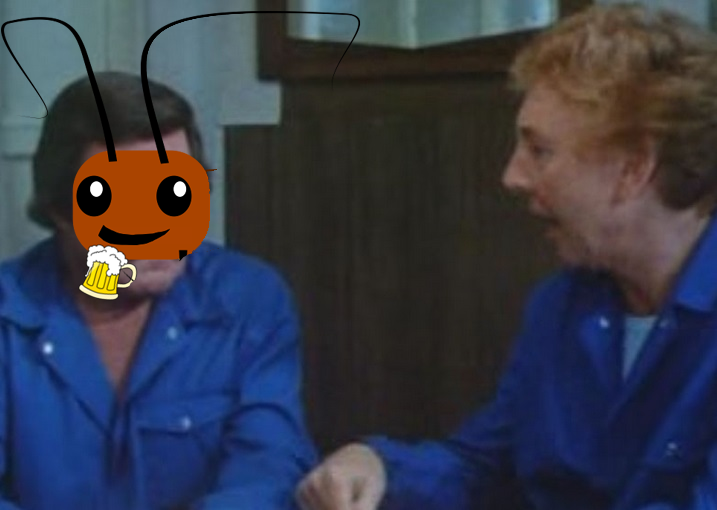
\includegraphics[scale=0.40]{1}}
\end{center}
\begin{flushleft}
\makebox[\textwidth]{Volledige naam:\enspace\hrulefill}
\end{flushleft} }
\question[2] {
\begin{center}
{
\includegraphics[scale=0.20]{2}}
\end{center}
\begin{flushleft}
\makebox[\textwidth]{naam:\enspace\hrulefill}
\end{flushleft} }
\question[1] {
\begin{center}
{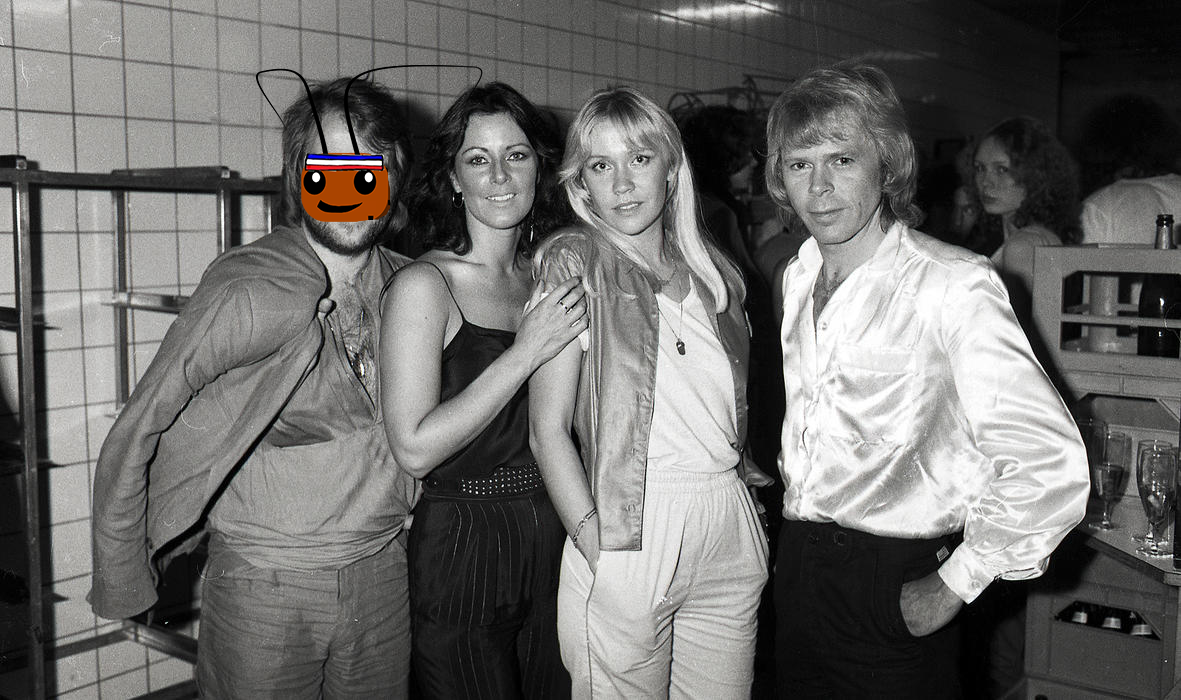
\includegraphics[scale=0.30]{3}}
\end{center}
\begin{flushleft}
\makebox[\textwidth]{naam:\enspace\hrulefill}
\end{flushleft} }
\question[1] {
\begin{center}
{
\includegraphics[scale=0.15]{4}}
\end{center}
\begin{flushleft}
\makebox[\textwidth]{naam:\enspace\hrulefill}
\end{flushleft} }
\question[1] {
\begin{center}
{
\includegraphics[scale=0.80]{5}}
\end{center}
\begin{flushleft}
\makebox[\textwidth]{naam:\enspace\hrulefill}
\end{flushleft} }

\question[3]{
{
\begin{table}[h]
\centering
\begin{tabular}{llll}
\textbf{Amerikaan} & \textbf{Verbranding}          & \textbf{Rapper} & \textbf{Nummer}    \\
\textbf{Zweepslag}      & \textbf{Van voor naar achter} & \textbf{Acteur}       & \textbf{Genie in Aladdin }   \\
\textbf{Auschwitz} & \textbf{Letsel}           & \textbf{Joden}          & \textbf{Nek}
\end{tabular}
\end{table}
}
\begin{flushleft}
\makebox[\textwidth]{Link 1:\enspace\hrulefill\linebreak}
\makebox[\textwidth]{Link 2:\enspace\hrulefill}
\makebox[\textwidth]{Link 3:\enspace\hrulefill}
\end{flushleft}
}

\question[3]{
{\begin{table}[h]
\centering
\begin{tabular}{llll}
\textbf{VTM} & \textbf{Citroen}          & \textbf{Brussel} & \textbf{Sunrise}    \\
\textbf{CSI}      & \textbf{Parijs} & \textbf{Mexicaans}       & \textbf{The Simpsons}   \\
\textbf{London} & \textbf{Zout}           & \textbf{Amsterdam}          & \textbf{Temptation Island }
\end{tabular}
\end{table}
}
\begin{flushleft}
\makebox[\textwidth]{Link 1:\enspace\hrulefill}
\makebox[\textwidth]{Link 2:\enspace\hrulefill}
\makebox[\textwidth]{Link 3:\enspace\hrulefill}
\end{flushleft}
}

\question[3]{
{\begin{table}[h]
\centering
\begin{tabular}{llll}
\textbf{Bieten} & \textbf{Klein}          & \textbf{De pil} & \textbf{Condoom}    \\
\textbf{Kristalstructuur}      & \textbf{Spielberg} & \textbf{Pessarium}       & \textbf{Telefoneren}   \\
\textbf{Riet} & \textbf{Buitenaards}           & \textbf{CH20}          & \textbf{Spiraaltje}
\end{tabular}
\end{table}
}
\begin{flushleft}
\makebox[\textwidth]{Link 1:\enspace\hrulefill}
\makebox[\textwidth]{Link 2:\enspace\hrulefill}
\makebox[\textwidth]{Link 3:\enspace\hrulefill}
\end{flushleft}
}
\newpage
\question[3]{
{\begin{table}[h]
\centering
\begin{tabular}{llll}
\textbf{Dagboek} & \textbf{Papier}          & \textbf{Joods meisje} & \textbf{Bezem}    \\
\textbf{Onderduiken}      & \textbf{Kraanvogel} & \textbf{Brandstapel}       & \textbf{Japans}   \\
\textbf{Vouwen} & \textbf{vrouw}           & \textbf{Schuilhuis}          & \textbf{Neuswrat}
\end{tabular}
\end{table}
}
\begin{flushleft}
\makebox[\textwidth]{Link 1:\enspace\hrulefill}
\makebox[\textwidth]{Link 2:\enspace\hrulefill}
\makebox[\textwidth]{Link 3:\enspace\hrulefill}
\end{flushleft}
}
\question[3]{
{\begin{table}[h]
\centering
\begin{tabular}{llll}
\textbf{Neuswrat} & \textbf{rapper}          & \textbf{brandstapel} & \textbf{papier}    \\
\textbf{Amerikaan}      & \textbf{Kraanvogel} & \textbf{bezem}       & \textbf{genie in Alladin}   \\
\textbf{vouwen} & \textbf{vrouw}           & \textbf{Acteur}          & \textbf{Japans}
\end{tabular}
\end{table}
}
\begin{flushleft}
\makebox[\textwidth]{Link 1:\enspace\hrulefill}
\makebox[\textwidth]{Link 2:\enspace\hrulefill}
\makebox[\textwidth]{Link 3:\enspace\hrulefill}
\end{flushleft}
}

\end{questions}

\begin{table}[!b]
\centering
\begin{tabular}{|l|l|l|l|l|l|l|l|l|l|l|l}
\hline
Vraag       & 1 & 2 & 3 & 4 & 5 & 6 & 7 & 8 & 9 & 10 \\ \hline
max. punten & 1 & 1 & 1 & 1 & 1 & 3 & 3 & 3 & 3 & 3\\ \hline
score       &   &   &   &   &   &   &   &   &   &  \\ \hline
\end{tabular}
\end{table}
\newpage
%
\section{Tafel ronde 2: Wie is het?}
Freddy heeft een paar mooie foto's gevonden van het home Astrid presidium. Kan jij raden wie het is?

Enkel voornaam, fonentisch geschreven
\begin{questions}
\question[1] {
\begin{center}
{\includegraphics[scale=0.20]{robbe}}
\end{center}
\begin{flushleft}
\makebox[\textwidth]{naam:\enspace\hrulefill}
\end{flushleft} }
\question[1] {
\begin{center}
{\includegraphics[scale=0.08]{lisa}}
\end{center}
\begin{flushleft}
\makebox[\textwidth]{naam:\enspace\hrulefill}
\end{flushleft} }
\question[1] {
\begin{center}
{\includegraphics[scale=0.20]{arend}}
\end{center}
\begin{flushleft}
\makebox[\textwidth]{naam:\enspace\hrulefill}
\end{flushleft} }
\question[1] {
\begin{center}
{\includegraphics[scale=0.10]{bart}}
\end{center}
\begin{flushleft}
\makebox[\textwidth]{naam:\enspace\hrulefill}
\end{flushleft} }
\question[1] {
\begin{center}
{\includegraphics[scale=0.20]{michelle}}
\end{center}
\begin{flushleft}
\makebox[\textwidth]{naam:\enspace\hrulefill}
\end{flushleft} }
\question[1] {
\begin{center}
{\includegraphics[scale=0.40]{lemmy}}
\end{center}
\begin{flushleft}
\makebox[\textwidth]{naam:\enspace\hrulefill}
\end{flushleft} }
\question[1] {
\begin{center}
{\includegraphics[scale=0.40]{tibo}}
\end{center}
\begin{flushleft}
\makebox[\textwidth]{naam:\enspace\hrulefill}
\end{flushleft} }
\question[1] {
\begin{center}
{\includegraphics[scale=0.10]{wouter}}
\end{center}
\begin{flushleft}
\makebox[\textwidth]{naam:\enspace\hrulefill}
\end{flushleft} }
\question[1] {
\begin{center}
{\includegraphics[scale=0.40]{elien}}
\end{center}
\begin{flushleft}
\makebox[\textwidth]{naam:\enspace\hrulefill}
\end{flushleft} }
\question[1] {
\begin{center}
{\includegraphics[scale=0.10]{sander}}
\end{center}
\begin{flushleft}
\makebox[\textwidth]{naam:\enspace\hrulefill}
\end{flushleft} }

\end{questions}

\begin{table}[!b]
\centering
\begin{tabular}{|l|l|l|l|l|l|l|l|l|l|l|l}
\hline
Vraag       & 1 & 2 & 3 & 4 & 5 & 6 & 7 & 8 & 9 & 10 \\ \hline
max. punten & 1 & 1 & 1 & 1 & 1 & 1 & 1 & 1 & 1 & 1 \\ \hline
score       &   &   &   &   &   &   &   &   &   &   \\ \hline
\end{tabular}
\end{table}
\newpage
%\section{Tafel ronde 3: raadsel ronde}
\begin{questions}
\question[4] {\begin{flushleft}
{\large Raadsel 1: Twenty-one}
\end{flushleft}
\begin{flushleft}
Dit raadsel komt van de thuisstad van Tibo (cultuur home Astrid). In Koksijde staan er veel wetgevingen op hoogte bouw, dus is er maar één echt super hoog gebouw: de Twenty-one. Rara-ra, het gebouw heeft 21 verdiepen. Nu woont de beste vriend van Freddy op de 21ste verdieping. Elke dag als het mooi weer is neemt hij de lift naar beneden en de trap naar boven. Echter wanneer het slecht weer is neemt hij de lift naar beneden en ook de lift naar boven.
\linebreak
De vraag is, hoe komt dit? Waarom neemt hij niet altijd de lift?
\linebreak
\end{flushleft}
}
\it Hint: op slechte dagen neemt hij een paraplu mee!
\fillwithlines{\stretch{1}}
%raadsel 2
\question[2]{\begin{flushleft}
{\large Raadsel 2: Vogel}
\end{flushleft} Maak een vogel door 2 rechte strepen te plaatsen.\center
\includegraphics[scale=1]{kip}}
\newpage
\question[2]{\begin{flushleft}
{\large Raadsel 3: converteer het symbool naar een decimaal getal.}
\end{flushleft}
\begin{center}
\includegraphics[scale=0.4]{76}
\end{center}
\fillwithlines{2em}
}


\question[2] {\begin{flushleft}
{\large Raadsel 4: Ontcijfer}
\end{flushleft}
\begin{flushleft}
Ontcijfer deze boodschap!
\end{flushleft}
\begin{center}
Oleacahoydnebp xef 4
\end{center}
\it Hint! Kijk naar het nummer van het raadsel!
\fillwithlines{3em}
}

\newpage
\question[2] {\begin{flushleft}
{\large Raadsel 4: Symbolen}
\end{flushleft}
Bepaal de volgende symbolen (mintens 2 aanvullen ,maar maximum 5).
\center
\includegraphics[scale=1]{symbolen}
}



\question[2]{\begin{flushleft}
{\large Raadsel 6: Freddy probeert 8 konoginnnen op een schaakbord te zetten, zonder dat ze elkaar in de weg staan. Een koningin kan elke kant uit, dus ze kan horizontaal, verticaal en diagonaal bewegen. }
\end{flushleft}
\begin{center}

\includegraphics[scale=0.03]{schaakbord2}
\end{center}
\newpage
\question[4]{
Er zijn 4 verschillende dozen gegeven, telkens met bijhorend opschrift:

\vspace{0.2cm}

Doos A: \framebox[0.4\textwidth][l]{Het punt zit niet in doos B}

\vspace{0.2cm}

Doos B: \framebox[0.4\textwidth][l]{Het punt zit niet in doos C}

\vspace{0.2cm}

Doos C: \framebox[0.4\textwidth][l]{Het punt zit in doos D}

\vspace{0.2cm}

Doos D: \framebox[0.4\textwidth][l]{Het punt zit in doos A}
\vspace{0.2cm}

Er is maar één doos die de waarheid spreekt.
Je mag maar 1 doos kiezen en openen! 

\textbf{Er is een wiskundige manier voor deze vraag! men kan dit formaliseren met proposities en eventueel verzamelingenleer.}

{\em Opmerking:} om alle punten te krijgen moet je ook proposities geven!}
}
\newpage
\question[2]{
Er rijd een zwarte auto op een zwarte baan, de gebouwen zijn zwart en de bewoners hebben hun zwarte gordijnen gesloten. De autolichten en straatverlichting zijn gedooft. De auto stopt en laat de zwarte kat oversteken. Hoe komt het dat de autobestuurder de zwarte kat zag?

\fillwithlines{\stretch{1}}
}
\end{questions}
\begin{table}[!b]
\centering
\begin{tabular}{|l|l|l|l|l|l|l|l|l|l|l|}
\hline
Vraag       & 1 & 2 & 3 & 4 & 5 & 6 & 7 & 8 \\ \hline
max. punten & 4 & 2 & 2 & 2 & 2 & 2 & 4 & 2 \\ \hline
score       &   &   &   &   &   &   &   &   \\ \hline
\end{tabular}
\end{table}

\end{document}